
%% bare_conf.tex
%% V1.3
%% 2007/01/11
%% by Michael Shell
%% See:
%% http://www.michaelshell.org/
%% for current contact information.
%%
%% This is a skeleton file demonstrating the use of IEEEtran.cls
%% (requires IEEEtran.cls version 1.7 or later) with an IEEE conference paper.
%%
%% Support sites:
%% http://www.michaelshell.org/tex/ieeetran/
%% http://www.ctan.org/tex-archive/macros/latex/contrib/IEEEtran/
%% and
%% http://www.ieee.org/

%%*************************************************************************
%% Legal Notice:
%% This code is offered as-is without any warranty either expressed or
%% implied; without even the implied warranty of MERCHANTABILITY or
%% FITNESS FOR A PARTICULAR PURPOSE!
%% User assumes all risk.
%% In no event shall IEEE or any contributor to this code be liable for
%% any damages or losses, including, but not limited to, incidental,
%% consequential, or any other damages, resulting from the use or misuse
%% of any information contained here.
%%
%% All comments are the opinions of their respective authors and are not
%% necessarily endorsed by the IEEE.
%%
%% This work is distributed under the LaTeX Project Public License (LPPL)
%% ( http://www.latex-project.org/ ) version 1.3, and may be freely used,
%% distributed and modified. A copy of the LPPL, version 1.3, is included
%% in the base LaTeX documentation of all distributions of LaTeX released
%% 2003/12/01 or later.
%% Retain all contribution notices and credits.
%% ** Modified files should be clearly indicated as such, including  **
%% ** renaming them and changing author support contact information. **
%%
%% File list of work: IEEEtran.cls, IEEEtran_HOWTO.pdf, bare_adv.tex,
%%                    bare_conf.tex, bare_jrnl.tex, bare_jrnl_compsoc.tex
%%*************************************************************************

% *** Authors should verify (and, if needed, correct) their LaTeX system  ***
% *** with the testflow diagnostic prior to trusting their LaTeX platform ***
% *** with production work. IEEE's font choices can trigger bugs that do  ***
% *** not appear when using other class files.                            ***
% The testflow support page is at:
% http://www.michaelshell.org/tex/testflow/



% Note that the a4paper option is mainly intended so that authors in
% countries using A4 can easily print to A4 and see how their papers will
% look in print - the typesetting of the document will not typically be
% affected with changes in paper size (but the bottom and side margins will).
% Use the testflow package mentioned above to verify correct handling of
% both paper sizes by the user's LaTeX system.
%
% Also note that the "draftcls" or "draftclsnofoot", not "draft", option
% should be used if it is desired that the figures are to be displayed in
% draft mode.
%
\documentclass[a4paper,conference]{IEEEtran}
\usepackage[utf8]{inputenc}
% Add the compsoc option for Computer Society conferences.
%
% If IEEEtran.cls has not been installed into the LaTeX system files,
% manually specify the path to it like:
% \documentclass[conference]{../sty/IEEEtran}





% Some very useful LaTeX packages include:
% (uncomment the ones you want to load)


% *** MISC UTILITY PACKAGES ***
%
%\usepackage{ifpdf}
% Heiko Oberdiek's ifpdf.sty is very useful if you need conditional
% compilation based on whether the output is pdf or dvi.
% usage:
% \ifpdf
%   % pdf code
% \else
%   % dvi code
% \fi
% The latest version of ifpdf.sty can be obtained from:
% http://www.ctan.org/tex-archive/macros/latex/contrib/oberdiek/
% Also, note that IEEEtran.cls V1.7 and later provides a builtin
% \ifCLASSINFOpdf conditional that works the same way.
% When switching from latex to pdflatex and vice-versa, the compiler may
% have to be run twice to clear warning/error messages.






% *** CITATION PACKAGES ***
%
\usepackage{cite}
% cite.sty was written by Donald Arseneau
% V1.6 and later of IEEEtran pre-defines the format of the cite.sty package
% \cite{} output to follow that of IEEE. Loading the cite package will
% result in citation numbers being automatically sorted and properly
% "compressed/ranged". e.g., [1], [9], [2], [7], [5], [6] without using
% cite.sty will become [1], [2], [5]--[7], [9] using cite.sty. cite.sty's
% \cite will automatically add leading space, if needed. Use cite.sty's
% noadjust option (cite.sty V3.8 and later) if you want to turn this off.
% cite.sty is already installed on most LaTeX systems. Be sure and use
% version 4.0 (2003-05-27) and later if using hyperref.sty. cite.sty does
% not currently provide for hyperlinked citations.
% The latest version can be obtained at:
% http://www.ctan.org/tex-archive/macros/latex/contrib/cite/
% The documentation is contained in the cite.sty file itself.






% *** GRAPHICS RELATED PACKAGES ***
%
\ifCLASSINFOpdf
  \usepackage[pdftex]{graphicx}
  % declare the path(s) where your graphic files are
  \graphicspath{{./images/}}
  % and their extensions so you won't have to specify these with
  % every instance of \includegraphics
  \DeclareGraphicsExtensions{.pdf,.jpeg,.png,.jpg}
\else
  % or other class option (dvipsone, dvipdf, if not using dvips). graphicx
  % will default to the driver specified in the system graphics.cfg if no
  % driver is specified.
  % \usepackage[dvips]{graphicx}
  % declare the path(s) where your graphic files are
  % \graphicspath{{../eps/}}
  % and their extensions so you won't have to specify these with
  % every instance of \includegraphics
  % \DeclareGraphicsExtensions{.eps}
\fi
% graphicx was written by David Carlisle and Sebastian Rahtz. It is
% required if you want graphics, photos, etc. graphicx.sty is already
% installed on most LaTeX systems. The latest version and documentation can
% be obtained at:
% http://www.ctan.org/tex-archive/macros/latex/required/graphics/
% Another good source of documentation is "Using Imported Graphics in
% LaTeX2e" by Keith Reckdahl which can be found as epslatex.ps or
% epslatex.pdf at: http://www.ctan.org/tex-archive/info/
%
% latex, and pdflatex in dvi mode, support graphics in encapsulated
% postscript (.eps) format. pdflatex in pdf mode supports graphics
% in .pdf, .jpeg, .png and .mps (metapost) formats. Users should ensure
% that all non-photo figures use a vector format (.eps, .pdf, .mps) and
% not a bitmapped formats (.jpeg, .png). IEEE frowns on bitmapped formats
% which can result in "jaggedy"/blurry rendering of lines and letters as
% well as large increases in file sizes.
%
% You can find documentation about the pdfTeX application at:
% http://www.tug.org/applications/pdftex





% *** MATH PACKAGES ***
%
%\usepackage[cmex10]{amsmath}
% A popular package from the American Mathematical Society that provides
% many useful and powerful commands for dealing with mathematics. If using
% it, be sure to load this package with the cmex10 option to ensure that
% only type 1 fonts will utilized at all point sizes. Without this option,
% it is possible that some math symbols, particularly those within
% footnotes, will be rendered in bitmap form which will result in a
% document that can not be IEEE Xplore compliant!
%
% Also, note that the amsmath package sets \interdisplaylinepenalty to 10000
% thus preventing page breaks from occurring within multiline equations. Use:
%\interdisplaylinepenalty=2500
% after loading amsmath to restore such page breaks as IEEEtran.cls normally
% does. amsmath.sty is already installed on most LaTeX systems. The latest
% version and documentation can be obtained at:
% http://www.ctan.org/tex-archive/macros/latex/required/amslatex/math/





% *** SPECIALIZED LIST PACKAGES ***
%
%\usepackage{algorithmic}
% algorithmic.sty was written by Peter Williams and Rogerio Brito.
% This package provides an algorithmic environment fo describing algorithms.
% You can use the algorithmic environment in-text or within a figure
% environment to provide for a floating algorithm. Do NOT use the algorithm
% floating environment provided by algorithm.sty (by the same authors) or
% algorithm2e.sty (by Christophe Fiorio) as IEEE does not use dedicated
% algorithm float types and packages that provide these will not provide
% correct IEEE style captions. The latest version and documentation of
% algorithmic.sty can be obtained at:
% http://www.ctan.org/tex-archive/macros/latex/contrib/algorithms/
% There is also a support site at:
% http://algorithms.berlios.de/index.html
% Also of interest may be the (relatively newer and more customizable)
% algorithmicx.sty package by Szasz Janos:
% http://www.ctan.org/tex-archive/macros/latex/contrib/algorithmicx/




% *** ALIGNMENT PACKAGES ***
%
%\usepackage{array}
% Frank Mittelbach's and David Carlisle's array.sty patches and improves
% the standard LaTeX2e array and tabular environments to provide better
% appearance and additional user controls. As the default LaTeX2e table
% generation code is lacking to the point of almost being broken with
% respect to the quality of the end results, all users are strongly
% advised to use an enhanced (at the very least that provided by array.sty)
% set of table tools. array.sty is already installed on most systems. The
% latest version and documentation can be obtained at:
% http://www.ctan.org/tex-archive/macros/latex/required/tools/


%\usepackage{mdwmath}
%\usepackage{mdwtab}
% Also highly recommended is Mark Wooding's extremely powerful MDW tools,
% especially mdwmath.sty and mdwtab.sty which are used to format equations
% and tables, respectively. The MDWtools set is already installed on most
% LaTeX systems. The lastest version and documentation is available at:
% http://www.ctan.org/tex-archive/macros/latex/contrib/mdwtools/


% IEEEtran contains the IEEEeqnarray family of commands that can be used to
% generate multiline equations as well as matrices, tables, etc., of high
% quality.


%\usepackage{eqparbox}
% Also of notable interest is Scott Pakin's eqparbox package for creating
% (automatically sized) equal width boxes - aka "natural width parboxes".
% Available at:
% http://www.ctan.org/tex-archive/macros/latex/contrib/eqparbox/





% *** SUBFIGURE PACKAGES ***
%\usepackage[tight,footnotesize]{subfigure}
% subfigure.sty was written by Steven Douglas Cochran. This package makes it
% easy to put subfigures in your figures. e.g., "Figure 1a and 1b". For IEEE
% work, it is a good idea to load it with the tight package option to reduce
% the amount of white space around the subfigures. subfigure.sty is already
% installed on most LaTeX systems. The latest version and documentation can
% be obtained at:
% http://www.ctan.org/tex-archive/obsolete/macros/latex/contrib/subfigure/
% subfigure.sty has been superceeded by subfig.sty.



%\usepackage[caption=false]{caption}
%\usepackage[font=footnotesize]{subfig}
% subfig.sty, also written by Steven Douglas Cochran, is the modern
% replacement for subfigure.sty. However, subfig.sty requires and
% automatically loads Axel Sommerfeldt's caption.sty which will override
% IEEEtran.cls handling of captions and this will result in nonIEEE style
% figure/table captions. To prevent this problem, be sure and preload
% caption.sty with its "caption=false" package option. This is will preserve
% IEEEtran.cls handing of captions. Version 1.3 (2005/06/28) and later
% (recommended due to many improvements over 1.2) of subfig.sty supports
% the caption=false option directly:
%\usepackage[caption=false,font=footnotesize]{subfig}
%
% The latest version and documentation can be obtained at:
% http://www.ctan.org/tex-archive/macros/latex/contrib/subfig/
% The latest version and documentation of caption.sty can be obtained at:
% http://www.ctan.org/tex-archive/macros/latex/contrib/caption/




% *** FLOAT PACKAGES ***
%
%\usepackage{fixltx2e}
% fixltx2e, the successor to the earlier fix2col.sty, was written by
% Frank Mittelbach and David Carlisle. This package corrects a few problems
% in the LaTeX2e kernel, the most notable of which is that in current
% LaTeX2e releases, the ordering of single and double column floats is not
% guaranteed to be preserved. Thus, an unpatched LaTeX2e can allow a
% single column figure to be placed prior to an earlier double column
% figure. The latest version and documentation can be found at:
% http://www.ctan.org/tex-archive/macros/latex/base/

\usepackage{subfig}

%\usepackage{stfloats}
% stfloats.sty was written by Sigitas Tolusis. This package gives LaTeX2e
% the ability to do double column floats at the bottom of the page as well
% as the top. (e.g., "\begin{figure*}[!b]" is not normally possible in
% LaTeX2e). It also provides a command:
%\fnbelowfloat
% to enable the placement of footnotes below bottom floats (the standard
% LaTeX2e kernel puts them above bottom floats). This is an invasive package
% which rewrites many portions of the LaTeX2e float routines. It may not work
% with other packages that modify the LaTeX2e float routines. The latest
% version and documentation can be obtained at:
% http://www.ctan.org/tex-archive/macros/latex/contrib/sttools/
% Documentation is contained in the stfloats.sty comments as well as in the
% presfull.pdf file. Do not use the stfloats baselinefloat ability as IEEE
% does not allow \baselineskip to stretch. Authors submitting work to the
% IEEE should note that IEEE rarely uses double column equations and
% that authors should try to avoid such use. Do not be tempted to use the
% cuted.sty or midfloat.sty packages (also by Sigitas Tolusis) as IEEE does
% not format its papers in such ways.





% *** PDF, URL AND HYPERLINK PACKAGES ***
%
%\usepackage{url}
% url.sty was written by Donald Arseneau. It provides better support for
% handling and breaking URLs. url.sty is already installed on most LaTeX
% systems. The latest version can be obtained at:
% http://www.ctan.org/tex-archive/macros/latex/contrib/misc/
% Read the url.sty source comments for usage information. Basically,
% \url{my_url_here}.





% *** Do not adjust lengths that control margins, column widths, etc. ***
% *** Do not use packages that alter fonts (such as pslatex).         ***
% There should be no need to do such things with IEEEtran.cls V1.6 and later.
% (Unless specifically asked to do so by the journal or conference you plan
% to submit to, of course. )


% correct bad hyphenation here
\hyphenation{op-tical net-works semi-conduc-tor}


\begin{document}
%
% paper title
% can use linebreaks \\ within to get better formatting as desired
\title{P2P Security - State of the Art\\
Forschungsmethoden WS2012\\
Gruppe 7}

% author names and affiliations
% use a multiple column layout for up to three different
% affiliations
\author{0502196 - Andreas Rohner\\
%0828266 - Murat Dogan\\
%1029102 - Christian Marbach\\
0626885 - Andreas Egger
}

% conference papers do not typically use \thanks and this command
% is locked out in conference mode. If really needed, such as for
% the acknowledgment of grants, issue a \IEEEoverridecommandlockouts
% after \documentclass

% for over three affiliations, or if they all won't fit within the width
% of the page, use this alternative format:
%
%\author{\IEEEauthorblockN{Michael Shell\IEEEauthorrefmark{1},
%Homer Simpson\IEEEauthorrefmark{2},
%James Kirk\IEEEauthorrefmark{3},
%Montgomery Scott\IEEEauthorrefmark{3} and
%Eldon Tyrell\IEEEauthorrefmark{4}}
%\IEEEauthorblockA{\IEEEauthorrefmark{1}School of Electrical and Computer Engineering\\
%Georgia Institute of Technology,
%Atlanta, Georgia 30332--0250\\ Email: see http://www.michaelshell.org/contact.html}
%\IEEEauthorblockA{\IEEEauthorrefmark{2}Twentieth Century Fox, Springfield, USA\\
%Email: homer@thesimpsons.com}
%\IEEEauthorblockA{\IEEEauthorrefmark{3}Starfleet Academy, San Francisco, California 96678-2391\\
%Telephone: (800) 555--1212, Fax: (888) 555--1212}
%\IEEEauthorblockA{\IEEEauthorrefmark{4}Tyrell Inc., 123 Replicant Street, Los Angeles, California 90210--4321}}




% use for special paper notices
%\IEEEspecialpapernotice{(Invited Paper)}




% make the title area
\maketitle

\begin{abstract}
A P2P approach seems to be the next logical step for many services that have to
scale massivly like VoIP. But a P2P service implies new security challenges
since clients have to rely on untrusted peers. It is difficult to identify
malicious peers without central control. This paper describes a selection of
possible security threats in this
environment, and then discusses some approaches, presented in the scientific
literature, to ameliorate them. Since the list of possible threats is extensive and the space in this paper is limited,
we focuses on only a selection of possible attacks.
\end{abstract}

\section{Introduction}

P2P applications face a number of security threats, because it has
to rely on untrusted and possibly malicious peers to provide the service.

Furthermore private data such as offline messages and voice mails have to be
stored in the overlay network and therefore on untrusted peers, who can
deny access to it or return fake content. Contact information, such as the
current ip address of the node, and other metadata is typically stored in the
overlay network as well.

In the case of a P2P VoIP application, a malicious peer who is
responsible for storing that kind of information could log all incoming calls or
prevent the user from getting any calls at all
\cite{touceda}.

% In section \ref{relatedwork} related work is discussed and
% section \ref{p2p} gives an overview of P2P VoIP in general and of a selection
% of possible attacks. \textsc{Touceda et al.} \cite{touceda} provide a recent
% complete survey of this
% topic. There are numerous possible attacks of the P2P overlay and the impact
% of most attacks can be mitigated by a carefully designed system, but for the
% purpose of this paper especially those attacks,
% that require some kind of user interaction, were chosen. In section
% \ref{usablesecurity} a new approach to mobile security proposed by
% \textsc{Toninelli et al.} \cite{toninelli} is discussed
%  and the findings of \textsc{Koskela et al.} \cite{koskela} are summarized in
% reference to the attacks presented in section \ref{p2p}. Section
% \ref{conclusion} tries to draw some conclusions.

\section{Security Threats for P2P VoIP}
\label{p2p}
In an P2P VoIP network the clients have to rely on untrusted peers to provide
the service. This makes it difficult to identify malicious peers, which can
manipulate
the network or provide false information. This section describes a selection of
security threats, that usually require the users attention.

\subsection{P2P architecture}
\begin{figure}
\centering
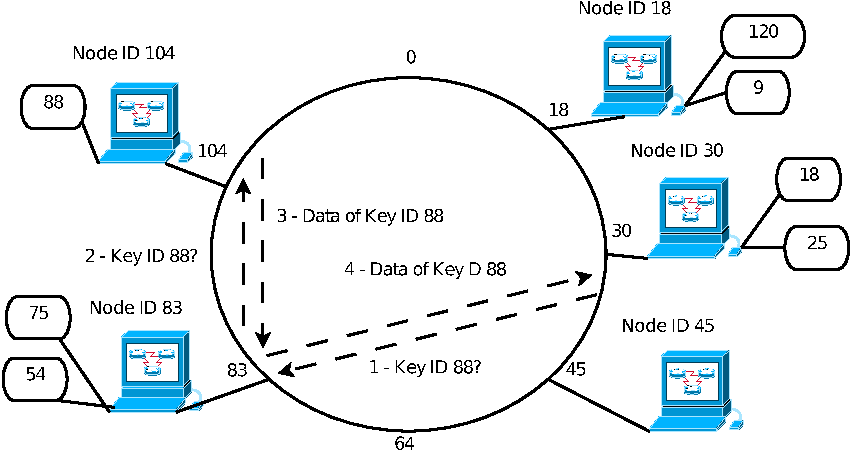
\includegraphics[width=0.5\textwidth]{p2p}

\caption{P2P overlay network \cite{touceda}}
\label{fig:p2p}
\end{figure}

P2P networks can be classified as either structured or unstructured, whereby the
latter tend to be relatively simple with inefficient searching and the former
use
a distributed hash table (DHT) \cite{chopra}. For the purposes of VoIP a
structured approach seems to be more appropriate because an
efficient lookup is needed. So the attacks described in this section assume a
structured overlay network.


Usually a hash function is used to hash keys into the key space, which is formed
by all possible results of the hash function. Every participant of the overlay
network has a unique random id, which determines the part of the key space it is
responsible for. The ids are of the same size
as the output of the hash function. If a peer wants to store a key value pair in
the DHT it sends the value to the peer, whose id is nearest to the hashed key.
To lookup a key in the DHT it sends a message to the
node in its routing table, whose id is nearest to the hashed key, which in turn
routes the message to the nearest node in its routing table.
Since every node knows its immediate neighborhood, the node responsible for the
key can be found very quickly.

In figure \ref{fig:p2p} node 30 does a lookup of key 88. It queries the nearest
node in its routing table, which happens to be node 83. Node 83 routes the
request to node 104, which is responsible for key 88 and returns the data for
it.

In a simple design malicious nodes can easily disrupt the routing process or
manipulate the values and therefore most implementations use a
public key infrastructure to encrypt and sign the messages. \textsc{Touceda et
al.} \cite{touceda} provide a very good overview of all possible attacks on P2P
VoIP systems.

\subsection{ID Mapping Attack}
\label{idmap}
Usually a node stores its resources in the overlay network, using the hash of
its username as a key. In a P2P VoIP network mostly the nodes contact
information, but
 also voice mails and offline messages are stored. If a node A wants to contact
another node B it hashes its username and does a lookup to retrieve the
contact information, which is stored at a third possibly malicious node C, whose
id is nearest to the hashed username.

So admission control is the first line of defense and very important for the
whole security of the network \cite{touceda, chopra}.
Because if a node can choose its id freely, it can position itself at an
arbitrary spot in the overlay network and make itself responsible for the
resources of a legitimate node. That way it can easily monitor incoming calls,
deny access to it or return fake information \cite{touceda}. Multiple attackers
could also position themselves in such a way, that they appear in the routing
table of the target node. Thereby they could completely manipulate the target
nodes view
of the network.

A simple solution would be to use the hash of the ip address as node id, but,
apart from being incompatible with NATs, where multiple nodes share a single
public ip,
it would still be possible for an attacker, who has access to a large range of
ips, to find a hash near the target key space. Since the key space
is much larger than the number of nodes it suffices to get an id that is near to
the targets hashed username \cite{touceda}.
Another solution would be to use a central certificate authority, which assigns
the node ids at random and signs them with its private key.


\subsection{Sybil Attack}
\label{sybil}
\begin{figure}
\centering
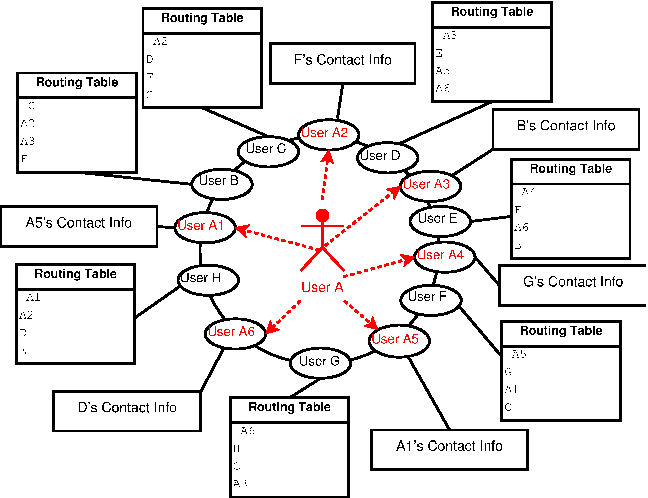
\includegraphics[width=0.5\textwidth]{sybil}

\caption{Sybil attack where user A controls the network with multiple identities
\cite{touceda}}
\label{fig:sybil}
\end{figure}
Even if a user is not allowed to choose his node id freely, if there is no limit
on the number of ids he can obtain, a sybil attack is possible.
In that case one attacker could present itself to the system with an unlimited
number of ids and thereby take over a huge part of the overlay network, by
appearing in the routing tables of legitimate users or controlling their contact
information.
It can be shown, that if there is no central control a sybil attack is always
possible \cite{douceur, touceda}.

In figure \ref{fig:sybil} user A presents himself to the network with multiple
node ids and thereby gets control over all contact information and appears in
the routing tables of all other users multiple times.

To prevent this attack the node id could depend on the ip address, which limits
the number of fake nodes to the number of ip addresses available to the
attacker. But
as stated in section \ref{idmap} this approach comes with its own problems. On
the other hand a central certificate authority could link the
node ids with some personal identification such as passport number or social
security number. But it would prove difficult to explain to the end users
why they are required to identify themselves to the certificate authority.

\subsection{Communications Log Attack}
\label{comlog}
\begin{figure}
\centering
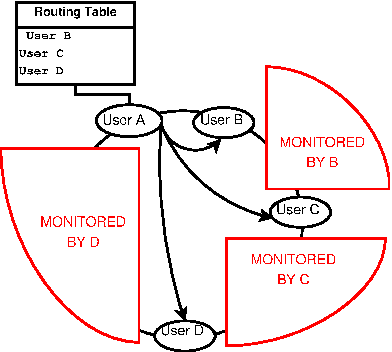
\includegraphics[width=0.5\textwidth]{log}

\caption{Key space which can be monitored by the users in A's routing table
\cite{touceda}}
\label{fig:log}
\end{figure}
Since a node accesses the network through the members of its routing table,
these nodes can monitor all communications. Figure \ref{fig:log} shows a node A
with
nodes B, C and D in its routing table. So
B, C and D can monitor all lookups of A in the key space between them, because A
uses them to route the requests into their respective key spaces. All
nodes on the path from A to the target can also log the message or tamper with
it if it is not encrypted and signed.

As was also noted in section \ref{idmap} an attacker who is responsible for
storing the contact information of a legitimate user can monitor all
incoming calls or deny access to the data, preventing anyone to call the node.

One way to make this attack harder is to use slightly randomized routing
mechanisms, so that not always the same path is chosen. This of course
reduces the efficiency of the routing process. Another way is to obfuscate the
message headers so that they don't reveal anything about the route of
the message \cite{touceda}.
Additionally to prevent an attacker from surrounding a node, id mapping and
sybil attacks described in sections \ref{idmap} and \ref{sybil} respectively
have
to be prevented \cite{touceda}.

Even if all these nodes were trustworthy the contact information of a node is
publicly available and can trivially be accessed through a lookup
\cite{koskelaold}.
So every node in the network can inquire the status of a user and his ip.
Because a P2P network relies on the close cooperation of its participants
it is difficult to provide privacy for the users \cite{koskelaold}.

\subsection{Eclipse Attack}
\label{eclipse}
An eclipse attack is more general attack that can be launched against the whole network using one or a combination of some of the attacks previously described.
In an Eclipse Attack, an attacker tries to mediate most overlay traffic in order to eclipse legit users from each others’ view \cite{touceda}. If an attacker
can control the users view of the network and all the incomming and outgoing traffic, he can perfom various forms of denail of service attacks. There are
mutliple ways of performing an eclipse attack, with different combinations of other attacks, but since this paper does not discuss all of these, so we
limit ourselves to the combination of sybil and ID mapping.

If an attacker can chose its id freely, as described in section \ref{idmap}, it can position itself strategically in the network and appear in the routing
tables of most of the users, as described in section \ref{sybil}. This means that most of the traffic is routed through the attacker and it can arbitraily deny
access to data or monitor activities of the users.

\subsection{Spam}
\label{spam}
To avoid the same situation as with email, P2P VoIP systems have to be designed
to cope with spam or unsolicited messages and calls. The first step to this end
would be a good admission control as stated in section \ref{idmap} to limit the
number of identities a spam bot can control \cite{touceda}, because, as we see
with email,
if it is easy to obtain or fake new identities, it is hard to prevent spam.
There are three different kinds of spam. Spam over instant messages or SPIM,
spam over
presence protocol or SPPP and spam over ip telephony or SPIT \cite{touceda}.
Whereby SPIT is a much greater disturbance than email spam, because emails can
be filtered based on content on the server before they reach the user, but
unsolicited calls require the immediate attention of the user and cannot be
filtered
based on content until they are answered \cite{heikkilae}. The list below
summarizes some of the more interesting defenses against spam taken from
\cite{touceda}.

\subsubsection{Grey Lists}
If a node contacts another node for the first time it is put on the grey list
and the call is refused with the remark to try again later.
A normal node would try again after a few seconds and the user might not even
notice a difference to a normal call, but a spam bot cannot afford to lose those
seconds per call.
This approach is already known to work well with emails.

\subsubsection{Turing Tests}
To ensure that a human being is behind every call turing tests or CAPTCHAs can
be used. These tests challenge the caller to do something
humans can do, but computers currently cannot. In the case of VoIP, voice based
CAPTCHAs would be used, but any kind
of CAPTCHA would do, such as the distorted images we know from websites.

\subsubsection{Computational Puzzles}
If user A contacts user B, B responds with a computational puzzle and wont
process user A's request until it receives a correct answer \cite{touceda}. Such
puzzles
are difficult to compute, but easy to check, making it computationally expensive
for an attacker to call a large number of addresses in a short time.
But since many different devices with different resources participate in the
network the complexity of these puzzles have to be rather low, which
reduces the effectiveness of this defense.

\subsubsection{Payments at Risk}
If user A calls user B, A transfers a small amount of money to B. If it is a
legitimate call B returns the money, but if it is SPIT B keeps it. Although
the amounts would be very small the accumulated cost of calling thousands of
people would make SPIT very expensive. It is not clear how this money transfer
can reliably work without contacting a central server and thereby losing the
advantages of a decentralized system.


\section{Related Work}
\label{relatedwork}

\textsc{Lua et al.} \cite{lua} provide a good survey and comparison of available
P2P overlay networks and \textsc{Wallach} \cite{wallach} gives an overview of
security threats
and attacks of P2P systems.

\textsc{Germanus et al.} \cite{germanus} investigate possibilites to ameliorate Localized Eclipse Attacks (LEA) on P2P Systems. They propose heuristics to
asses the suceptibility of various P2P protocols to LEA attacks based on routing mechanisms and topology characteristics. The results can be used to tune the
parameters of these networks and improve their resilience. The Localized Eclipse Attack is a form of Eclipse Attack described in section \ref{eclipse}.


\section{Conclusion}
\label{conclusion}
In this paper a brief introduction into P2P overlay networks, in reference to
P2P VoIP, was given and a summary of some of the attacks, that could exploit
this
architecture followed. Then the usability implications of the defenses and
recent developments in the field of usable security were discussed. It seems,
that
the advantages of a P2P architecture, like scalability and fault tolerance, come
at a price, because the dependence on untrusted peers leaves the user
vulnerable to attacks. Securing P2P networks is a difficult task and an active
field of research. Most of the scientific literature agrees, that at least
some form of central certificate authority, that performs admission control, is
necessary to prevent an attacker from choosing its id freely or get an unlimited
number of fake ids. This measure mitigates many attacks and strengthens the
effectiveness of reputation and social link systems.

% use section* for acknowledgement
%\section*{Acknowledgment}


% An example of a floating figure using the graphicx package.
% Note that \label must occur AFTER (or within) \caption.
% For figures, \caption should occur after the \includegraphics.
% Note that IEEEtran v1.7 and later has special internal code that
% is designed to preserve the operation of \label within \caption
% even when the captionsoff option is in effect. However, because
% of issues like this, it may be the safest practice to put all your
% \label just after \caption rather than within \caption{}.
%
% Reminder: the "draftcls" or "draftclsnofoot", not "draft", class
% option should be used if it is desired that the figures are to be
% displayed while in draft mode.
%
%\begin{figure}[!t]
%\centering
%\includegraphics{lala}

%\caption{Simulation Results}
%\end{figure}

% Note that IEEE typically puts floats only at the top, even when this
% results in a large percentage of a column being occupied by floats.


% An example of a double column floating figure using two subfigures.
% (The subfig.sty package must be loaded for this to work.)
% The subfigure \label commands are set within each subfloat command, the
% \label for the overall figure must come after \caption.
% \hfil must be used as a separator to get equal spacing.
% The subfigure.sty package works much the same way, except \subfigure is
% used instead of \subfloat.
%
%\begin{figure*}[!t]
%\centerline{\subfloat[Case I]\includegraphics[width=2.5in]{subfigcase1}%
%\label{fig_first_case}}
%\hfil
%\subfloat[Case II]{\includegraphics[width=2.5in]{subfigcase2}%
%\label{fig_second_case}}}
%\caption{Simulation results}
%\label{fig_sim}
%\end{figure*}
%
% Note that often IEEE papers with subfigures do not employ subfigure
% captions (using the optional argument to \subfloat), but instead will
% reference/describe all of them (a), (b), etc., within the main caption.


% An example of a floating table. Note that, for IEEE style tables, the
% \caption command should come BEFORE the table. Table text will default to
% \footnotesize as IEEE normally uses this smaller font for tables.
% The \label must come after \caption as always.
%
%\begin{table}[!t]
%% increase table row spacing, adjust to taste
%\renewcommand{\arraystretch}{1.3}
% if using array.sty, it might be a good idea to tweak the value of
% \extrarowheight as needed to properly center the text within the cells
%\caption{An Example of a Table}
%\label{table_example}
%\centering
%% Some packages, such as MDW tools, offer better commands for making tables
%% than the plain LaTeX2e tabular which is used here.
%\begin{tabular}{|c||c|}
%\hline
%One & Two\\
%\hline
%Three & Four\\
%\hline
%\end{tabular}
%\end{table}


% Note that IEEE does not put floats in the very first column - or typically
% anywhere on the first page for that matter. Also, in-text middle ("here")
% positioning is not used. Most IEEE journals/conferences use top floats
% exclusively. Note that, LaTeX2e, unlike IEEE journals/conferences, places
% footnotes above bottom floats. This can be corrected via the \fnbelowfloat
% command of the stfloats package.







% conference papers do not normally have an appendix






% trigger a \newpage just before the given reference
% number - used to balance the columns on the last page
% adjust value as needed - may need to be readjusted if
% the document is modified later
%\IEEEtriggeratref{8}
% The "triggered" command can be changed if desired:
%\IEEEtriggercmd{\enlargethispage{-5in}}

% references section

% can use a bibliography generated by BibTeX as a .bbl file
% BibTeX documentation can be easily obtained at:
% http://www.ctan.org/tex-archive/biblio/bibtex/contrib/doc/
% The IEEEtran BibTeX style support page is at:
% http://www.michaelshell.org/tex/ieeetran/bibtex/
\bibliographystyle{IEEEtran}
% argument is your BibTeX string definitions and bibliography database(s)
\bibliography{IEEEabrv,references}
%
% <OR> manually copy in the resultant .bbl file
% set second argument of \begin to the number of references
% (used to reserve space for the reference number labels box)
%\begin{thebibliography}{1}

%\bibitem{IEEEhowto:kopka}
%H.~Kopka and P.~W. Daly, \emph{A Guide to \LaTeX}, 3rd~ed.\hskip 1em plus
%  0.5em minus 0.4em\relax Harlow, England: Addison-Wesley, 1999.

%\end{thebibliography}




% that's all folks
\end{document}


